\documentclass[a4paper]{article}

\usepackage{array}
\usepackage{listings}
\usepackage{appendix}
\usepackage{hyperref}
\usepackage{graphicx}
\usepackage{numprint}
\usepackage{booktabs}
\usepackage{subcaption}
\usepackage{listings}
\usepackage[T1]{fontenc}

\usepackage{hyperref}
\hypersetup{
  colorlinks=true,
  linkcolor=blue,
  filecolor=magenta,
  urlcolor=cyan,
}
\npdecimalsign{.}
\nprounddigits{4}

\title{Raijin to Gadi Transition Consistency Tests for Processing Sentinel-2 Collection 1}
\date{16 March 2020}
\author{Analysis Read Data\\ Pipelines and Data Workflows Team}

\begin{document}
  \pagenumbering{gobble}
  \maketitle
  \newpage
  \pagenumbering{arabic}

  \section{Introduction}

    \begin{flushleft}
      The National Computational Infrastructure (NCI) Australia is shutting down the Raijin compute cluster and moving to the Gadi compute cluster. This can have an impact on the consistency on data products, with the worst case scenario being the archive needs to be reprocessed. \par
      This report aims to present information regarding the consistency of the output products when using a different processing environment to output Digital Earth Australia's Sentinel-2 Collection 1 products. \par
      The report is not a reflection of the Gadi compute cluster, nor a suggestion that there is anything wrong with the Gadi compute cluster. \par
      Reports on the analytical findings regarding the consistency of any Collection level processing should be undertaken when setting up any new processing pipelines.
    \end{flushleft}

    \subsection{Processing environments}
    \label{sec:environ}
      \begin{itemize}
        \item Raijin
          \begin{itemize}
            \item 5.3.1 (Compiled with GCC-5.2.0)
            \item eugl-0.1.0
            \item tesp-0.5.2
            \item fmask-0.4.5
            \item gverify-0.25v
            \item MODTRAN-5.2.1
          \end{itemize}
        \item Gadi
          \begin{itemize}
            \item wagl-5.3.1.gadi (Compiled with GCC-8.2.1)
            \item eugl-0.1.0
            \item tesp-0.5.2.gadi
            \item fmask-0.4.5
            \item gverify-0.25v
            \item MODTRAN-5.2.1
          \end{itemize}
      \end{itemize}

    \subsection{Base input data}

      ESA Sentinel-2 L1C

    \subsection{Acquisition Period}

      2019/11/01 -> 2019/11/10

    \subsection{Reported Metrics}
      \begin{itemize}
        \item Minimum residual
        \item Maximum residual
        \item Percentage of pixels that are different
        \item Min and Max percentage of pixels that have changed categorical value
      \end{itemize}

    \subsection{Measurements}
      \begin{itemize}
        \item nbar\_coastal\_aerosol
        \item nbart\_coastal\_aerosol
        \item nbar\_blue
        \item nbart\_blue
        \item nbar\_green
        \item nbart\_green
        \item nbar\_red
        \item nbart\_red
        \item nbar\_red\_edge\_1
        \item nbar2\_red\_edge\_1
        \item nbar\_red\_edge\_2
        \item nbart\_red\_edge\_2
        \item nbar\_red\_edge\_3
        \item nbart\_red\_edge\_3
        \item nbar\_nir\_1
        \item nbart\_nir\_1
        \item nbar\_nir\_2
        \item nbart\_nir\_2
        \item nbar\_swir\_2
        \item nbart\_swir\_2
        \item nbar\_swir\_3
        \item nbart\_swir\_3
        \item fmask
        \item terrain\_shadow
        \item nbar\_contiguity
        \item nbart\_contiguity
        \item solar\_azimuth
        \item solar\_zenith
        \item azimuthal\_exiting
        \item azimuthal\_incident
        \item exiting
        \item incident
      \end{itemize}

    \subsection{Other Assessments}
      \begin{itemize}
        \item GQA (Geometric Quality Assessment)
        \item Software Versions
        \item File Naming Consistency
        \item Quicklook Images
      \end{itemize}

    \section{Method}

      \begin{flushleft}
        Sentinel-2 L1C acquisitions for the first 10 days for the month of November 2019 (approx 4700 granules) and processed on the Raijin compute cluster were used as input in the test production environment built on the Gadi compute cluster. \par
        The output product \textit{S2\_MSI\_ARD} processed on the Gadi compute cluster was then compared with the \textit{S2\_MSI\_ARD} product processed on the Raijin compute cluster.
      \end{flushleft}

    \subsection{Rationale}

      \begin{flushleft}
        Depending on the software versions being compared, it is expected that there will be change and the idea is to build a general understanding of the type of change that is occurring, be that large or small; not to define the explicit details of why a change has occurred. \par
        While extrema are reported (maximal and minimal residuals), they are often misinterpreted leading to biased assumptions as they don't describe the proportionality of change. The proportionality of change is what the aforementioned metrics are designed to describe. \par
        Initially, the metrics were designed to inform the operations team of a potential change in the underlying data, thus requiring further investigation and potentially leading to a recommendation to the leadership team for a collection upgrade. \par
        The percent different was simply describing the proportionality of change. For routine integration tests, it is ideal to have this number closer 0. As routine testing that is occurring on the same machine should exhibit less noise in floating point calculations. If deploying the codebase to a different machine, it is expected that there will be some floating point differences. This can occur due to slight differences in machine architecture, and/or different compilers. As such, this metric coupled with minimal and maximal differences/residuals, can help in aiding a user to ignore noise such as compiler or machine architecture differences. \par
      \end{flushleft}

  \newpage

  \section{Results}

    \subsection{Continental overview}

    \begin{flushleft}
      The following tables are reporting on the extrema (min and max) of difference for the different processing environments. \par
      The results for every acquisition within the first 10 days of the month of November 2019 are aggregated into their respective spatial regions and evaluated to find the total minimum and maximum of change in percent reflectance for a given measurement across the continent. \par
    \end{flushleft}

    \begin{table}[ht!]
      \caption{Minimum difference in surface reflectance (units are \% reflectance)}\label{table:1}
      \centering
      \begin{tabular}{cc} \midrule
        \textbf{Measurement} & \textbf{Minimum} \\ \midrule
        nbar\_coastal\_aerosol & -0.01 \\
        nbart\_coastal\_aerosol & -0.03 \\
        nbar\_blue & -0.01 \\
        nbart\_blue & -0.04 \\
        nbar\_green & -0.01 \\
        nbart\_green & -0.06 \\
        nbar\_red & -0.01 \\
        nbart\_red & -0.07 \\
        nbar\_red\_edge\_1 & -0.01 \\
        nbart\_red\_edge\_1 & -0.08 \\
        nbar\_red\_edge\_2 & -0.01 \\
        nbart\_red\_edge\_2 & -0.07 \\
        nbar\_red\_edge\_3 & -0.01 \\
        nbart\_red\_edge\_3 & -0.06 \\
        nbar\_nir\_1 & -0.01 \\
        nbart\_nir\_1 & -0.06 \\
        nbar\_nir\_2 & -0.01 \\
        nbart\_nir\_2 & -0.05 \\
        nbar\_swir\_2 & -0.01 \\
        nbart\_swir\_2 & -0.04 \\
        nbar\_swir\_3 & -0.01 \\
        nbart\_swir\_3 & -0.04 \\ \midrule
      \end{tabular}
    \end{table}

    \begin{table}[ht!]
      \caption{Maximum difference in surface reflectance (units are \% reflectance)}\label{table:2}
      \centering
      \begin{tabular}{cc} \midrule
        \textbf{Measurement} & \textbf{Maximum} \\ \midrule
        nbar\_coastal\_aerosol & 0.01 \\
        nbart\_coastal\_aerosol & 0.03 \\
        nbar\_blue & 0.01 \\
        nbart\_blue & 0.04 \\
        nbar\_green & 0.01 \\
        nbart\_green & 0.06 \\
        nbar\_red & 0.01 \\
        nbart\_red & 0.07 \\
        nbar\_red\_edge\_1 & 0.01 \\
        nbart\_red\_edge\_1 & 0.08 \\
        nbar\_red\_edge\_2 & 0.01 \\
        nbart\_red\_edge\_2 & 0.08 \\
        nbar\_red\_edge\_3 & 0.01 \\
        nbart\_red\_edge\_3 & 0.05 \\
        nbar\_nir\_1 & 0.01 \\
        nbart\_nir\_1 & 0.06 \\
        nbar\_nir\_2 & 0.01 \\
        nbart\_nir\_2 & 0.06 \\
        nbar\_swir\_2 & 0.01 \\
        nbart\_swir\_2 & 0.05 \\
        nbar\_swir\_3 & 0.01 \\
        nbart\_swir\_3 & 0.05 \\ \midrule
      \end{tabular}
    \end{table}

  \newpage

    \begin{table}[ht!]
      \caption{Maximum difference for the angular measurements (units are degrees)}\label{table:3}
      \centering
      \begin{tabular}{cc} \midrule
        \textbf{Measurement} & \textbf{Maximum} \\ \midrule
        solar\_azimuth & 7.659314178454224e-06 \\
        solar\_zenith & 1.914828544613556e-06 \\
        satellite\_azimuth & 3.0637256713816896e-05 \\
        satellite\_view & 1.3403799130173866e-05 \\
        azimuthal\_exiting & 362.8235168457031 \\
        azimuthal\_incident & 362.8235168457031 \\
        exiting & 0.08657556772232056 \\
        incident & 0.08689652383327484 \\ \midrule
      \end{tabular}
    \end{table}

  \clearpage

    \begin{flushleft}
      Table~\ref{table:4}, below, represents the proportion of pixels that a different (excluding those pixels that may have changed to a \textit{Null} or vice versa). The maximum percent of difference for each measurement is derived from a continental aggregation.
    \end{flushleft}

    \begin{table}[ht!]
      \caption{Percentage of pixels (acquisition wide) that are different}\label{table:4}
      \centering
      \begin{tabular}{cc} \midrule
        \textbf{Measurement} & \textbf{Percentage} \\ \midrule
        nbar\_coastal\_aerosol & 0.12322509684472405 \\
        nbart\_coastal\_aerosol & 0.1221001221001221 \\
        nbar\_blue & 0.11738654685994258 \\
        nbart\_blue & 0.11507637859154742 \\
        nbar\_green & 0.07305217965434753 \\
        nbart\_green & 0.10547742044651479 \\
        nbar\_red & 0.0983694425242626 \\
        nbart\_red & 0.11340622625671448 \\
        nbar\_red\_edge\_1 & 0.10273368821440922 \\
        nbart\_red\_edge\_1 & 0.11540107697054754 \\
        nbar\_red\_edge\_2 & 0.1260239445494644 \\
        nbart\_red\_edge\_2 & 0.11889476146396329, \\
        nbar\_red\_edge\_3 & 0.16703786191536749 \\
        nbart\_red\_edge\_3 & 0.12804097311139565 \\
        nbar\_nir\_1 & 0.1694915254237288 \\
        nbart\_nir\_1 & 0.11373552177995427 \\
        nbar\_nir\_2 & 0.07009598508299573 \\
        nbart\_nir\_2 & 0.11080586992080318 \\
        nbar\_swir\_2 & 0.06146281499692685 \\
        nbart\_swir\_2 & 0.13802622498274672 \\
        nbar\_swir\_3 & 0.057022448070423795 \\
        nbart\_swir\_3 & 0.09182736455463728 \\
        solar\_azimuth & 3.317839025086181e-06 \\
        solar\_zenith & 3.317839025086181e-06 \\
        satellite\_azimuth & 0.1269869708461485 \\
        satellite\_view & 25.497592907787297 \\
        azimuthal\_exiting & 10.43814055029678 \\
        azimuthal\_incident & 14.44151147474627 \\
        exiting\_angle & 17.807691414427953 \\
        incident\_angle & 31.77631792860674 \\ \midrule
      \end{tabular}
    \end{table}

      \begin{flushleft}
        The minimum and maximum difference are all reporting less than 1\% change in surface reflectance. \par
        This is unlikely to have a significant impact on DEA's products derived from this baseline. Aquatic remote sensing applications, such as suspended sediment concentration, may find this significant, however, it is recommended not to be using be using DEA's NBAR or NBART surface reflectance product for such applications. \par
        Applications identifying surface water may be less impacted than those measuring content within water bodies. \par
        The maximum proportion of differences for the surface reflectance bands is also less than 1\%, indicating minimal change from all acquisition over the continent for the first 10 days of the month of November 2019. \par
        For datasets containing angular measurements, there are large distribution of pixels that are different. However, as the minimal and maximal differences are quite small and have had little impact on the output surface reflectance, it is most likely due to differences in floating point calculations.
      \end{flushleft}

      \begin{flushleft}
        Table~\ref{table:5} and Table~\ref{table:6}, below, represents the minimum and maximum percentage of pixels in a given category within the Fmask schema changing to another category. i.e. Pixels originally classified as Clear and now being classified as Cloud. \par
        A value of 100 represents 100\%, and indicates that all pixels from all granules mapped entirely to the corresponding category. A NaN implies no recorded pixels for that category. \par
        A good indicator for data consistency for a category mapping to the same category, say cloud to cloud, is a value close to 100\%. For a category mapping to a different category, say cloud to snow, a value close to 0\% or NaN, is also good indicator for data consistency.
      \end{flushleft}

  \clearpage

    \begin{table}[ht!]
      \caption{Minimum percentage of categorical change within Fmask}\label{table:5}
      \centering
      \begin{tabular}{ccccccc} \midrule
        & \textbf{Null} & \textbf{Clear} & \textbf{Cloud} & \textbf{Cloud Shadow} & \textbf{Snow} & \textbf{Water} \\ \midrule
        \textbf{Null} & 100 & NaN & NaN & NaN & NaN & NaN \\
        \textbf{Clear} & NaN & 100 & NaN & NaN & NaN & NaN \\
        \textbf{Cloud} & NaN & NaN & 100 & NaN & NaN & NaN \\
        \textbf{Cloud Shadow} & NaN & NaN & NaN & 100 & NaN & NaN \\
        \textbf{Snow} & NaN & NaN & NaN & NaN & 100 & NaN \\
        \textbf{Water} & NaN & NaN & NaN & NaN & NaN & 100 \\
      \end{tabular}
    \end{table}

    \begin{table}[ht!]
      \caption{Maximum percentage of categorical change within Fmask}\label{table:6}
      \centering
      \begin{tabular}{ccccccc} \midrule
        & \textbf{Null} & \textbf{Clear} & \textbf{Cloud} & \textbf{Cloud Shadow} & \textbf{Snow} & \textbf{Water} \\ \midrule
        \textbf{Null} & 100 & NaN & NaN & NaN & NaN & NaN \\
        \textbf{Clear} & NaN & 100 & NaN & NaN & NaN & NaN \\
        \textbf{Cloud} & NaN & NaN & 100 & NaN & NaN & NaN \\
        \textbf{Cloud Shadow} & NaN & NaN & NaN & 100 & NaN & NaN \\
        \textbf{Snow} & NaN & NaN & NaN & NaN & 100 & NaN \\
        \textbf{Water} & NaN & NaN & NaN & NaN & NaN & 100 \\
      \end{tabular}
    \end{table}

      \begin{flushleft}
        As you can see, for the 10 days of acquisitions, covering the Australian continent, there is not a single pixel that has changed categorical states between the different processing environments.
      \end{flushleft}

  % \newpage

    \begin{flushleft}
      Table~\ref{table:7} and Table~\ref{table:8}, below, represents the minimum and maximum percentage of pixels, that are either contiguous or non-contiguous, changing from one category to another (or itself) \textit{nbart\_contiguity} measurement.
    \end{flushleft}

    \begin{table}[ht!]
      \caption{Minimum percentage of categorical change within the \textit{nbart\_contiguity} measurement}\label{table:7}
      \centering
      \begin{tabular}{ccc} \midrule
        & \textbf{Contiguous} & \textbf{Non-Contiguous} \\ \midrule
        \textbf{Contiguous} & 100.0 & NaN \\
        \textbf{Non-Contiguous} & NaN & 100 \\
      \end{tabular}
    \end{table}

    \begin{table}[ht!]
      \caption{Maximum percentage of categorical change within the \textit{nbart\_contiguity} measurement}\label{table:8}
      \centering
      \begin{tabular}{ccc} \midrule
        & \textbf{Contiguous} & \textbf{Non-Contiguous} \\ \midrule
        \textbf{Contiguous} & 100.0 & NaN \\
        \textbf{Non-Contiguous} & NaN & 100.0 \\
      \end{tabular}
    \end{table}

    \begin{flushleft}
      For the \textit{nbart\_contiguity} measurements, there is no categorical change for pixels between the two different processing environments.
    \end{flushleft}

    \begin{flushleft}
      Table~\ref{table:9} and Table~\ref{table:10}, below, represents the minimum and maximum percentage of pixels, that are either contiguous or non-contiguous, changing from one category to another (or itself) for the \textit{nbar\_contiguity} measurement.
    \end{flushleft}

    \begin{table}[ht!]
      \caption{Minimum percentage of categorical change within the \textit{oa\_nbar\_contiguity} measurement}\label{table:9}
      \centering
      \begin{tabular}{ccc} \midrule
        & \textbf{Contiguous} & \textbf{Non-Contiguous} \\ \midrule
        \textbf{Contiguous} & 100 & NaN \\
        \textbf{Non-Contiguous} & NaN & 100 \\
      \end{tabular}
    \end{table}

    \begin{table}[ht!]
      \caption{Maximum percentage of categorical change within the \textit{oa\_nbar\_contiguity} measurement}\label{table:10}
      \centering
      \begin{tabular}{ccc} \midrule
        & \textbf{Contiguous} & \textbf{Non-Contiguous} \\ \midrule
        \textbf{Contiguous} & 100.0 & NaN \\
        \textbf{Non-Contiguous} & NaN & 100.0 \\
      \end{tabular}
    \end{table}

    \begin{flushleft}
      For the \textit{nbar\_contiguity} measurement, there is no categorical change for pixels between the two different processing environments.
    \end{flushleft}

  % \vspace{5mm}
  \clearpage

    \begin{flushleft}
      Table~\ref{table:11} and Table~\ref{table:12}, below, represents the minimum and maximum percentage of pixels, that are either shadow or non-shadow, changing from one category to another (or itself) for the \textit{terrain\_shadow} measurement.
    \end{flushleft}

    \begin{table}[ht!]
      \caption{Minimum percentage of categorical change within the \textit{oa\_combined\_terrain\_shadow} measurement}\label{table:11}
      \centering
      \begin{tabular}{ccc} \midrule
        & \textbf{Shadow} & \textbf{Not-Shadow} \\ \midrule
        \textbf{Shadow} & 100.0 & NaN \\
        \textbf{Not-Shadow} & NaN & 100.0 \\
      \end{tabular}
    \end{table}

    \begin{table}[ht!]
      \caption{Maximum percentage of categorical change within the \textit{oa\_combined\_terrain\_shadow} measurement}\label{table:12}
      \centering
      \begin{tabular}{ccc} \midrule
        & \textbf{Shadow} & \textbf{Not-Shadow} \\ \midrule
        \textbf{Shadow} & 100.0 & NaN \\
        \textbf{Not-Shadow} & NaN & 100.0 \\
      \end{tabular}
    \end{table}

    \begin{flushleft}
      For the \textit{terrain\_shadow} measurement, there is no categorical change for pixels between the two different processing environments.
    \end{flushleft}

    \subsection{Spatial Distribution}

      \begin{flushleft}
        The following section presents the impact of change spatially across the continent. \par
        The idea is to pictorially represent whether there are any spatial patterns or associations with the changes in processing environments. \par
        This has an added advantage of informing users that while there might be change within the data collection that is being processed, their application may not be affected if differences are located in particular regions.
      \end{flushleft}

  \clearpage

    \subsubsection{Extrema Differences (\textit{min, max})}

      \begin{flushleft}
        The section is to present the spatial distribution of the residuals, and in particular, highlight the locations of extrema, and any spatial patterns that may be visible across the continent. \par
      \end{flushleft}

      \begin{figure}[h!]
        \centering
          \begin{subfigure}[l]{.4\linewidth}
            \hspace{-32mm}
            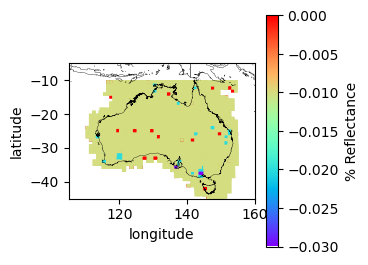
\includegraphics[scale=0.9]{plots/nbart/nbart_coastal_aerosol-MinResidual.png}
            \caption{Minimum residual}
          \end{subfigure}
%
          \begin{subfigure}[r]{.4\linewidth}
            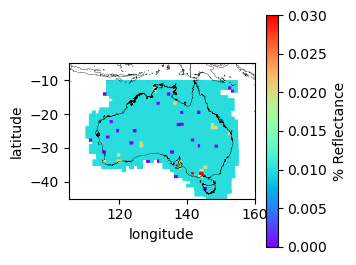
\includegraphics[scale=0.9]{plots/nbart/nbart_coastal_aerosol-MaxResidual.png}
            \caption{Maximum residual}
          \end{subfigure}
        \caption{NBART;\@ Coastal Aerosol Band}\label{figure:1}
      \end{figure}

      \begin{figure}[h!]
        \centering
          \begin{subfigure}[l]{.4\linewidth}
            \hspace{-32mm}
            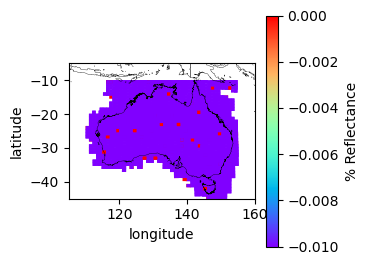
\includegraphics[scale=0.9]{plots/nbar/nbar_coastal_aerosol-MinResidual.png}
            \caption{Minimum residual}
          \end{subfigure}
%
          \begin{subfigure}[r]{.4\linewidth}
            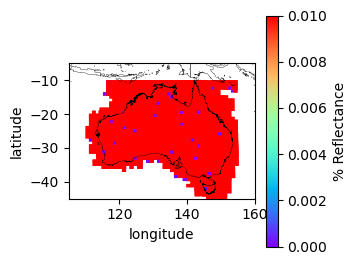
\includegraphics[scale=0.9]{plots/nbar/nbar_coastal_aerosol-MaxResidual.png}
            \caption{Maximum residual}
          \end{subfigure}
        \caption{NBAR;\@ Coastal Aerosol Band}\label{figure:2}
      \end{figure}

  \clearpage

      \begin{figure}[h!]
        \centering
          \begin{subfigure}[l]{.4\linewidth}
            \hspace{-32mm}
            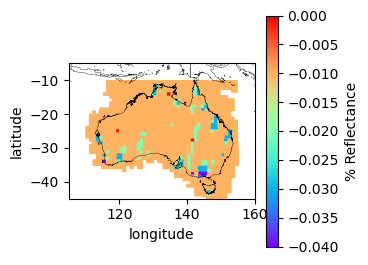
\includegraphics[scale=0.9]{plots/nbart/nbart_blue-MinResidual.png}
            \caption{Minimum residual}
          \end{subfigure}
%
          \begin{subfigure}[r]{.4\linewidth}
            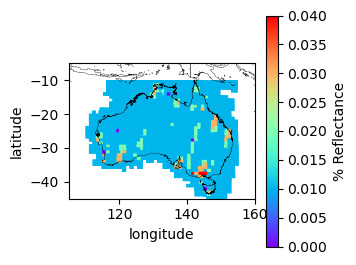
\includegraphics[scale=0.9]{plots/nbart/nbart_blue-MaxResidual.png}
            \caption{Maximum residual}
          \end{subfigure}
        \caption{NBART;\@ Blue Band}\label{figure:3}
      \end{figure}

      \begin{figure}[h!]
        \centering
          \begin{subfigure}[l]{.4\linewidth}
            \hspace{-32mm}
            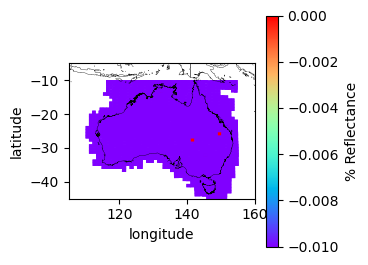
\includegraphics[scale=0.9]{plots/nbar/nbar_blue-MinResidual.png}
            \caption{Minimum residual}
          \end{subfigure}
%
          \begin{subfigure}[r]{.4\linewidth}
            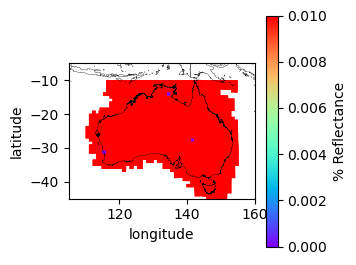
\includegraphics[scale=0.9]{plots/nbar/nbar_blue-MaxResidual.png}
            \caption{Maximum residual}
          \end{subfigure}
        \caption{NBAR;\@ Blue Band}\label{figure:4}
      \end{figure}

  \clearpage

      \begin{figure}[h!]
        \centering
          \begin{subfigure}[l]{.4\linewidth}
            \hspace{-32mm}
            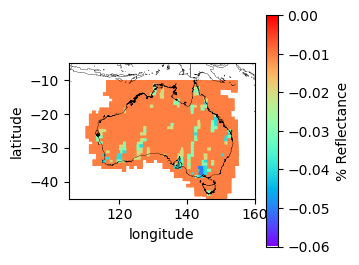
\includegraphics[scale=0.9]{plots/nbart/nbart_green-MinResidual.png}
            \caption{Minimum residual}
          \end{subfigure}
%
          \begin{subfigure}[r]{.4\linewidth}
            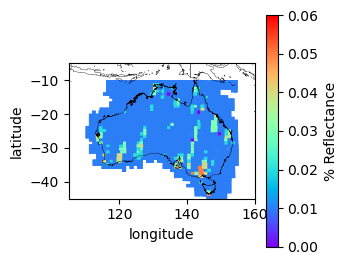
\includegraphics[scale=0.9]{plots/nbart/nbart_green-MaxResidual.png}
            \caption{Maximum residual}
          \end{subfigure}
        \caption{NBART;\@ Green Band}\label{figure:5}
      \end{figure}

      \begin{figure}[h!]
        \centering
          \begin{subfigure}[l]{.4\linewidth}
            \hspace{-32mm}
            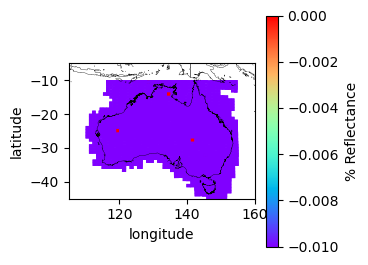
\includegraphics[scale=0.9]{plots/nbar/nbar_green-MinResidual.png}
            \caption{Minimum residual}
          \end{subfigure}
%
          \begin{subfigure}[r]{.4\linewidth}
            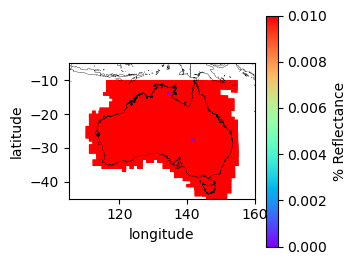
\includegraphics[scale=0.9]{plots/nbar/nbar_green-MaxResidual.png}
            \caption{Maximum residual}
          \end{subfigure}
        \caption{NBAR;\@ Green Band}\label{figure:6}
      \end{figure}

  \clearpage

      \begin{figure}[h!]
        \centering
          \begin{subfigure}[l]{.4\linewidth}
            \hspace{-32mm}
            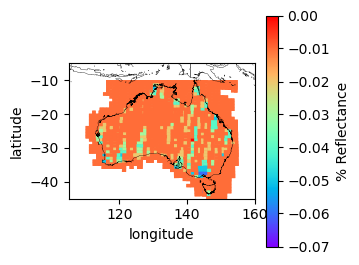
\includegraphics[scale=0.9]{plots/nbart/nbart_red-MinResidual.png}
            \caption{Minimum residual}
          \end{subfigure}
%
          \begin{subfigure}[r]{.4\linewidth}
            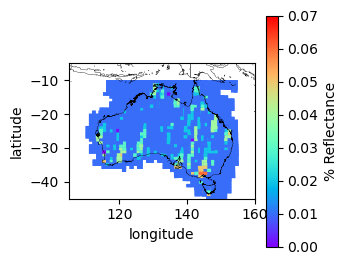
\includegraphics[scale=0.9]{plots/nbart/nbart_red-MaxResidual.png}
            \caption{Maximum residual}
          \end{subfigure}
        \caption{NBART;\@ Red Band}\label{figure:7}
      \end{figure}

      \begin{figure}[h!]
        \centering
          \begin{subfigure}[l]{.4\linewidth}
            \hspace{-32mm}
            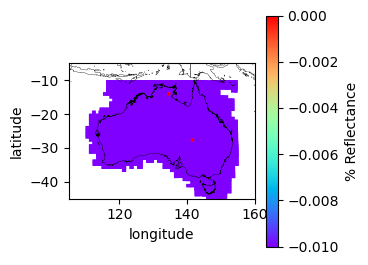
\includegraphics[scale=0.9]{plots/nbar/nbar_red-MinResidual.png}
            \caption{Minimum residual}
          \end{subfigure}
%
          \begin{subfigure}[r]{.4\linewidth}
            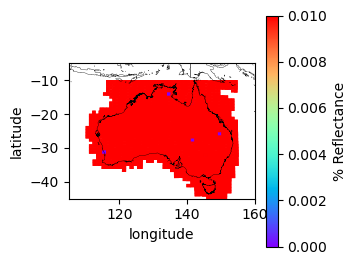
\includegraphics[scale=0.9]{plots/nbar/nbar_red-MaxResidual.png}
            \caption{Maximum residual}
          \end{subfigure}
        \caption{NBAR;\@ Red Band}\label{figure:8}
      \end{figure}

  \clearpage

      \begin{figure}[h!]
        \centering
          \begin{subfigure}[l]{.4\linewidth}
            \hspace{-32mm}
            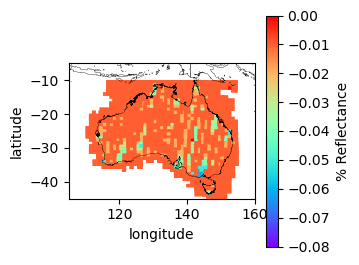
\includegraphics[scale=0.9]{plots/nbart/nbart_red_edge_1-MinResidual.png}
            \caption{Minimum residual}
          \end{subfigure}
%
          \begin{subfigure}[r]{.4\linewidth}
            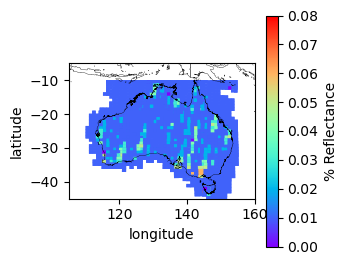
\includegraphics[scale=0.9]{plots/nbart/nbart_red_edge_1-MaxResidual.png}
            \caption{Maximum residual}
          \end{subfigure}
        \caption{NBART;\@ Red Edge 1 Band}\label{figure:9}
      \end{figure}

      \begin{figure}[h!]
        \centering
          \begin{subfigure}[l]{.4\linewidth}
            \hspace{-32mm}
            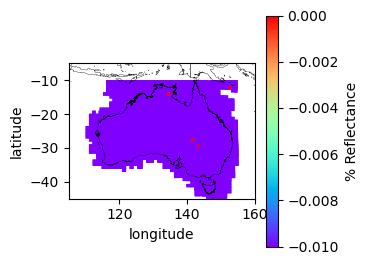
\includegraphics[scale=0.9]{plots/nbar/nbar_red_edge_1-MinResidual.png}
            \caption{Minimum residual}
          \end{subfigure}
%
          \begin{subfigure}[r]{.4\linewidth}
            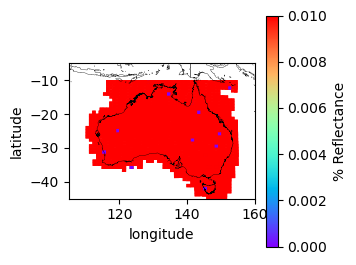
\includegraphics[scale=0.9]{plots/nbar/nbar_red_edge_1-MaxResidual.png}
            \caption{Maximum residual}
          \end{subfigure}
        \caption{NBAR;\@ Red Edge 1 Band}\label{figure:10}
      \end{figure}

  \clearpage

      \begin{figure}[h!]
        \centering
          \begin{subfigure}[l]{.4\linewidth}
            \hspace{-32mm}
            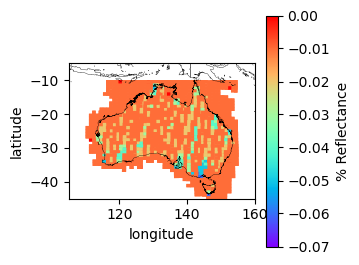
\includegraphics[scale=0.9]{plots/nbart/nbart_red_edge_2-MinResidual.png}
            \caption{Minimum residual}
          \end{subfigure}
%
          \begin{subfigure}[r]{.4\linewidth}
            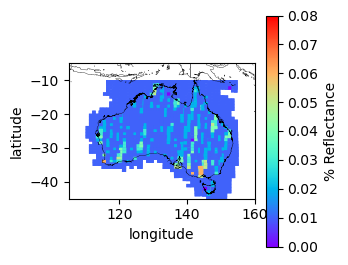
\includegraphics[scale=0.9]{plots/nbart/nbart_red_edge_2-MaxResidual.png}
            \caption{Maximum residual}
          \end{subfigure}
        \caption{NBART;\@ Red Edge 2 Band}\label{figure:11}
      \end{figure}

      \begin{figure}[h!]
        \centering
          \begin{subfigure}[l]{.4\linewidth}
            \hspace{-32mm}
            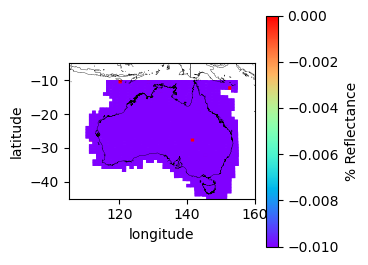
\includegraphics[scale=0.9]{plots/nbar/nbar_red_edge_2-MinResidual.png}
            \caption{Minimum residual}
          \end{subfigure}
%
          \begin{subfigure}[r]{.4\linewidth}
            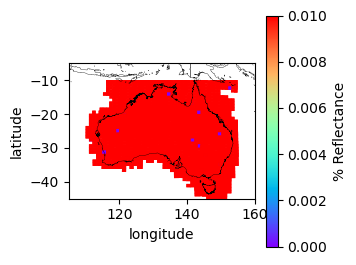
\includegraphics[scale=0.9]{plots/nbar/nbar_red_edge_2-MaxResidual.png}
            \caption{Maximum residual}
          \end{subfigure}
        \caption{NBAR;\@ Red Edge 2 Band}\label{figure:12}
      \end{figure}

  \clearpage

      \begin{figure}[h!]
        \centering
          \begin{subfigure}[l]{.4\linewidth}
            \hspace{-32mm}
            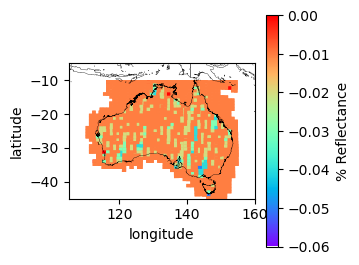
\includegraphics[scale=0.9]{plots/nbart/nbart_red_edge_3-MinResidual.png}
            \caption{Minimum residual}
          \end{subfigure}
%
          \begin{subfigure}[r]{.4\linewidth}
            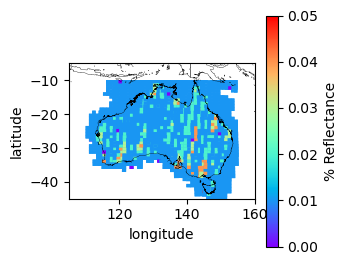
\includegraphics[scale=0.9]{plots/nbart/nbart_red_edge_3-MaxResidual.png}
            \caption{Maximum residual}
          \end{subfigure}
        \caption{NBART;\@ Red Edge 3 Band}\label{figure:13}
      \end{figure}

      \begin{figure}[h!]
        \centering
          \begin{subfigure}[l]{.4\linewidth}
            \hspace{-32mm}
            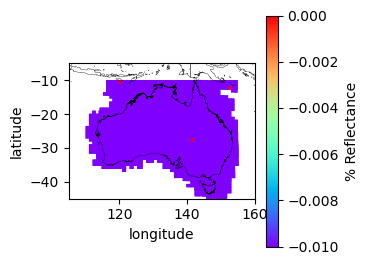
\includegraphics[scale=0.9]{plots/nbar/nbar_red_edge_3-MinResidual.png}
            \caption{Minimum residual}
          \end{subfigure}
%
          \begin{subfigure}[r]{.4\linewidth}
            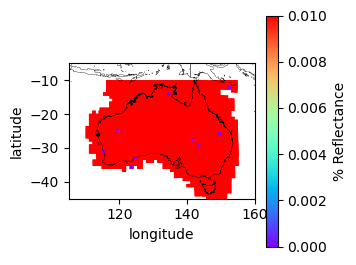
\includegraphics[scale=0.9]{plots/nbar/nbar_red_edge_3-MaxResidual.png}
            \caption{Maximum residual}
          \end{subfigure}
        \caption{NBAR;\@ Red Edge 3 Band}\label{figure:14}
      \end{figure}

  \clearpage

      \begin{figure}[h!]
        \centering
          \begin{subfigure}[l]{.4\linewidth}
            \hspace{-32mm}
            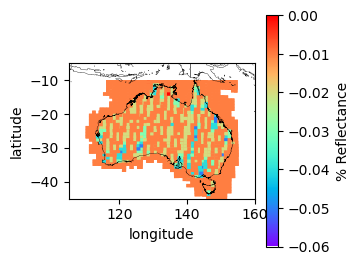
\includegraphics[scale=0.9]{plots/nbart/nbart_nir_1-MinResidual.png}
            \caption{Minimum residual}
          \end{subfigure}
%
          \begin{subfigure}[r]{.4\linewidth}
            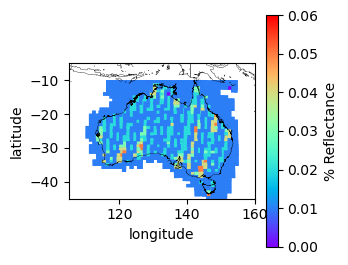
\includegraphics[scale=0.9]{plots/nbart/nbart_nir_1-MaxResidual.png}
            \caption{Maximum residual}
          \end{subfigure}
        \caption{NBART;\@ NIR-1 Band}\label{figure:15}
      \end{figure}

      \begin{figure}[h!]
        \centering
          \begin{subfigure}[l]{.4\linewidth}
            \hspace{-32mm}
            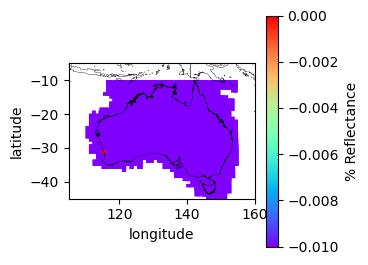
\includegraphics[scale=0.9]{plots/nbar/nbar_nir_1-MinResidual.png}
            \caption{Minimum residual}
          \end{subfigure}
%
          \begin{subfigure}[r]{.4\linewidth}
            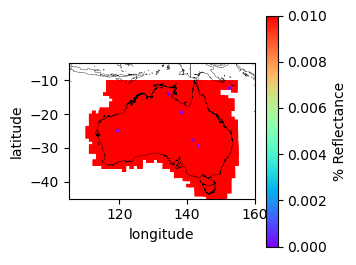
\includegraphics[scale=0.9]{plots/nbar/nbar_nir_1-MaxResidual.png}
            \caption{Maximum residual}
          \end{subfigure}
        \caption{NBAR;\@ NIR-1 Band}\label{figure:16}
      \end{figure}

  \clearpage

      \begin{figure}[h!]
        \centering
          \begin{subfigure}[l]{.4\linewidth}
            \hspace{-32mm}
            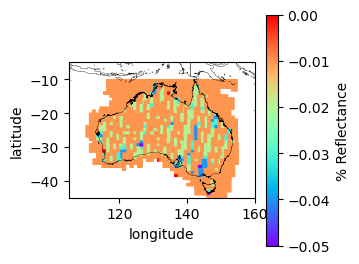
\includegraphics[scale=0.9]{plots/nbart/nbart_nir_2-MinResidual.png}
            \caption{Minimum residual}
          \end{subfigure}
%
          \begin{subfigure}[r]{.4\linewidth}
            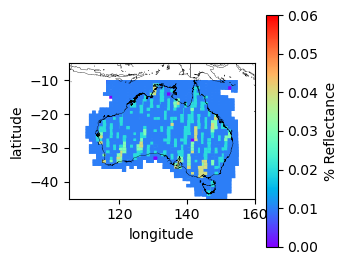
\includegraphics[scale=0.9]{plots/nbart/nbart_nir_2-MaxResidual.png}
            \caption{Maximum residual}
          \end{subfigure}
        \caption{NBART;\@ NIR-2 Band}\label{figure:17}
      \end{figure}

      \begin{figure}[h!]
        \centering
          \begin{subfigure}[l]{.4\linewidth}
            \hspace{-32mm}
            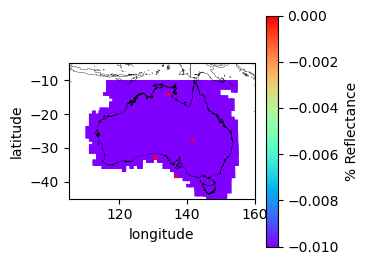
\includegraphics[scale=0.9]{plots/nbar/nbar_nir_2-MinResidual.png}
            \caption{Minimum residual}
          \end{subfigure}
%
          \begin{subfigure}[r]{.4\linewidth}
            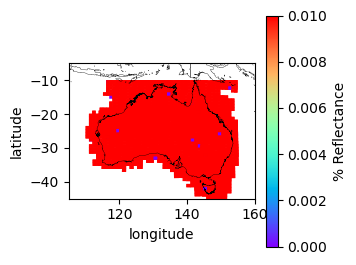
\includegraphics[scale=0.9]{plots/nbar/nbar_nir_2-MaxResidual.png}
            \caption{Maximum residual}
          \end{subfigure}
        \caption{NBAR;\@ NIR-2 Band}\label{figure:18}
      \end{figure}

  \clearpage

      \begin{figure}[h!]
        \centering
          \begin{subfigure}[l]{.4\linewidth}
            \hspace{-32mm}
            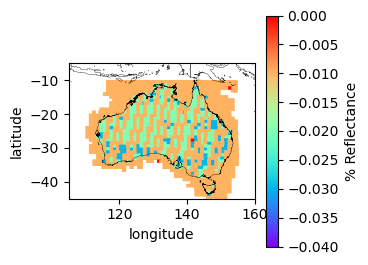
\includegraphics[scale=0.9]{plots/nbart/nbart_swir_2-MinResidual.png}
            \caption{Minimum residual}
          \end{subfigure}
%
          \begin{subfigure}[r]{.4\linewidth}
            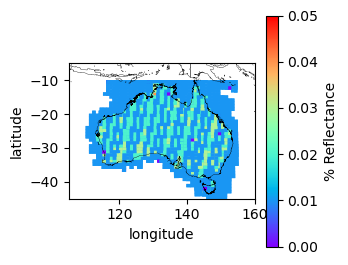
\includegraphics[scale=0.9]{plots/nbart/nbart_swir_2-MaxResidual.png}
            \caption{Maximum residual}
          \end{subfigure}
        \caption{NBART;\@ SWIR-2 Band}\label{figure:19}
      \end{figure}

      \begin{figure}[h!]
        \centering
          \begin{subfigure}[l]{.4\linewidth}
            \hspace{-32mm}
            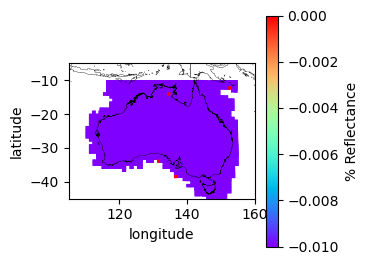
\includegraphics[scale=0.9]{plots/nbar/nbar_swir_2-MinResidual.png}
            \caption{Minimum residual}
          \end{subfigure}
%
          \begin{subfigure}[r]{.4\linewidth}
            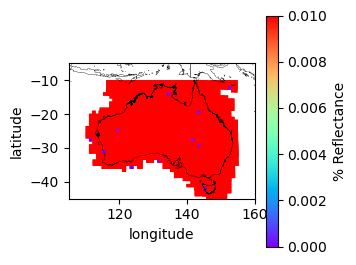
\includegraphics[scale=0.9]{plots/nbar/nbar_swir_2-MaxResidual.png}
            \caption{Maximum residual}
          \end{subfigure}
        \caption{NBAR;\@ SWIR-2 Band}\label{figure:20}
      \end{figure}

  \clearpage

      \begin{figure}[h!]
        \centering
          \begin{subfigure}[l]{.4\linewidth}
            \hspace{-32mm}
            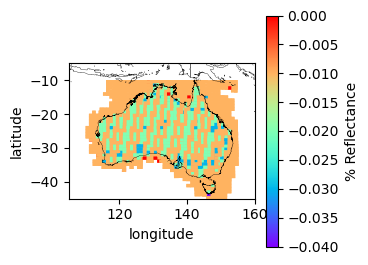
\includegraphics[scale=0.9]{plots/nbart/nbart_swir_3-MinResidual.png}
            \caption{Minimum residual}
          \end{subfigure}
%
          \begin{subfigure}[r]{.4\linewidth}
            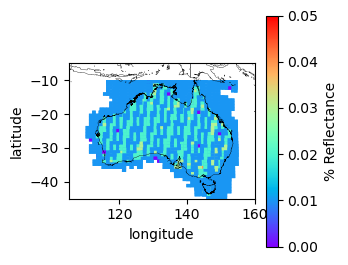
\includegraphics[scale=0.9]{plots/nbart/nbart_swir_3-MaxResidual.png}
            \caption{Maximum residual}
          \end{subfigure}
        \caption{NBART;\@ SWIR-3 Band}\label{figure:21}
      \end{figure}

      \begin{figure}[h!]
        \centering
          \begin{subfigure}[l]{.4\linewidth}
            \hspace{-32mm}
            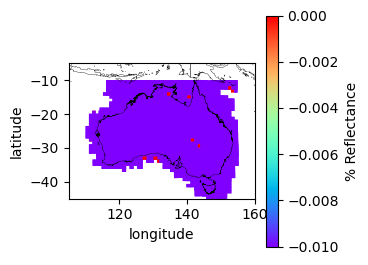
\includegraphics[scale=0.9]{plots/nbar/nbar_swir_3-MinResidual.png}
            \caption{Minimum residual}
          \end{subfigure}
%
          \begin{subfigure}[r]{.4\linewidth}
            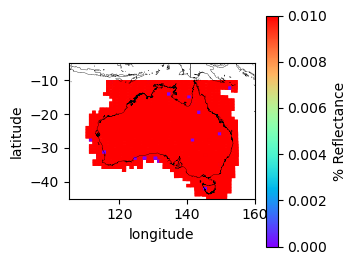
\includegraphics[scale=0.9]{plots/nbar/nbar_swir_3-MaxResidual.png}
            \caption{Maximum residual}
          \end{subfigure}
        \caption{NBAR;\@ SWIR-3 Band}\label{figure:22}
      \end{figure}

  \clearpage

    \subsubsection{Proportion of Differences (\textit{\% of pixels != 0})}

      \begin{flushleft}
        The section is to inform the spatial distribution of the proportionality of pixels that are different, i.e. the residual is != 0. \par
        Two key pieces of information can be inferred here:
        \begin{enumerate}
          \item The extremities for the proportion of non-zero residuals
          \item A spatial representation of non-zero residuals
        \end{enumerate}
      \end{flushleft}

      \begin{figure}[h!]
        \centering
          \begin{subfigure}[l]{.4\linewidth}
            \hspace{-32mm}
            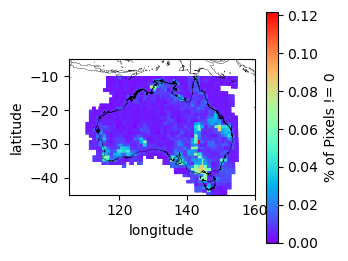
\includegraphics[scale=0.9]{plots/nbart/nbart_coastal_aerosol-PercentDifferent.png}
            \caption{NBART}
          \end{subfigure}
%
          \begin{subfigure}[r]{.4\linewidth}
            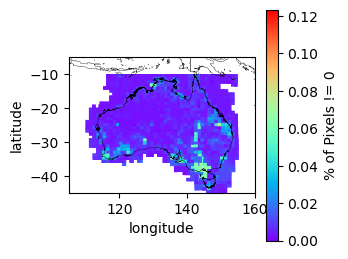
\includegraphics[scale=0.9]{plots/nbar/nbar_coastal_aerosol-PercentDifferent.png}
            \caption{NBAR}
          \end{subfigure}
        \caption{Coastal Aerosol Band \% Pixels != 0}\label{figure:23}
      \end{figure}

      \begin{figure}[h!]
        \centering
          \begin{subfigure}[l]{.4\linewidth}
            \hspace{-32mm}
            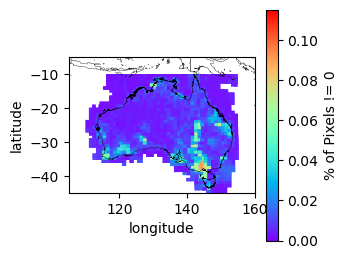
\includegraphics[scale=0.9]{plots/nbart/nbart_blue-PercentDifferent.png}
            \caption{NBART}
          \end{subfigure}
%
          \begin{subfigure}[r]{.4\linewidth}
            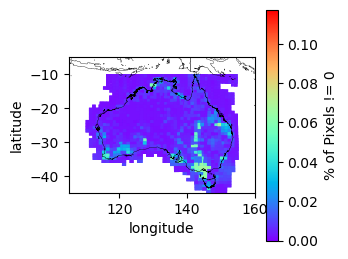
\includegraphics[scale=0.9]{plots/nbar/nbar_blue-PercentDifferent.png}
            \caption{NBAR}
          \end{subfigure}
        \caption{Blue Band \% Pixels != 0}\label{figure:24}
      \end{figure}

  \clearpage

      \begin{figure}[h!]
        \centering
          \begin{subfigure}[l]{.4\linewidth}
            \hspace{-32mm}
            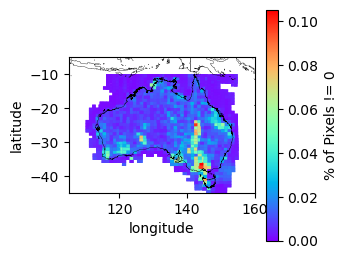
\includegraphics[scale=0.9]{plots/nbart/nbart_green-PercentDifferent.png}
            \caption{NBART}
          \end{subfigure}
%
          \begin{subfigure}[r]{.4\linewidth}
            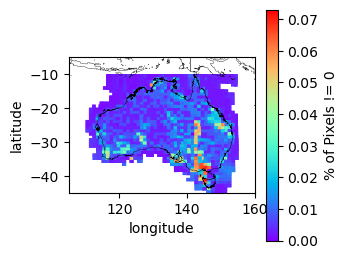
\includegraphics[scale=0.9]{plots/nbar/nbar_green-PercentDifferent.png}
            \caption{NBAR}
          \end{subfigure}
        \caption{Green Band \% Pixels != 0}\label{figure:25}
      \end{figure}

      \begin{figure}[h!]
        \centering
          \begin{subfigure}[l]{.4\linewidth}
            \hspace{-32mm}
            \includegraphics[scale=0.9]{plots/nbart/nbart_red-PercentDifferent.png}
            \caption{NBART}
          \end{subfigure}
%
          \begin{subfigure}[r]{.4\linewidth}
            \includegraphics[scale=0.9]{plots/nbar/nbar_red-PercentDifferent.png}
            \caption{NBAR}
          \end{subfigure}
        \caption{Red Band \% Pixels != 0}\label{figure:26}
      \end{figure}

  \clearpage

      \begin{figure}[h!]
        \centering
          \begin{subfigure}[l]{.4\linewidth}
            \hspace{-32mm}
            \includegraphics[scale=0.9]{plots/nbart/nbart_red_edge_1-PercentDifferent.png}
            \caption{NBART}
          \end{subfigure}
%
          \begin{subfigure}[r]{.4\linewidth}
            \includegraphics[scale=0.9]{plots/nbar/nbar_red_edge_1-PercentDifferent.png}
            \caption{NBAR}
          \end{subfigure}
        \caption{Red Edge 1 Band \% Pixels != 0}\label{figure:27}
      \end{figure}

      \begin{figure}[h!]
        \centering
          \begin{subfigure}[l]{.4\linewidth}
            \hspace{-32mm}
            \includegraphics[scale=0.9]{plots/nbart/nbart_red_edge_2-PercentDifferent.png}
            \caption{NBART}
          \end{subfigure}
%
          \begin{subfigure}[r]{.4\linewidth}
            \includegraphics[scale=0.9]{plots/nbar/nbar_red_edge_2-PercentDifferent.png}
            \caption{NBAR}
          \end{subfigure}
        \caption{Red Edge 2 Band \% Pixels != 0}\label{figure:28}
      \end{figure}

  \clearpage

      \begin{figure}[h!]
        \centering
          \begin{subfigure}[l]{.4\linewidth}
            \hspace{-32mm}
            \includegraphics[scale=0.9]{plots/nbart/nbart_red_edge_3-PercentDifferent.png}
            \caption{NBART}
          \end{subfigure}
%
          \begin{subfigure}[r]{.4\linewidth}
            \includegraphics[scale=0.9]{plots/nbar/nbar_red_edge_3-PercentDifferent.png}
            \caption{NBAR}
          \end{subfigure}
        \caption{Red Edge 3 Band \% Pixels != 0}\label{figure:29}
      \end{figure}

      \begin{figure}[h!]
        \centering
          \begin{subfigure}[l]{.4\linewidth}
            \hspace{-32mm}
            \includegraphics[scale=0.9]{plots/nbart/nbart_nir_1-PercentDifferent.png}
            \caption{NBART}
          \end{subfigure}
%
          \begin{subfigure}[r]{.4\linewidth}
            \includegraphics[scale=0.9]{plots/nbar/nbar_nir_1-PercentDifferent.png}
            \caption{NBAR}
          \end{subfigure}
        \caption{NIR-1 Band \% Pixels != 0}\label{figure:30}
      \end{figure}

  \clearpage

      \begin{figure}[h!]
        \centering
          \begin{subfigure}[l]{.4\linewidth}
            \hspace{-32mm}
            \includegraphics[scale=0.9]{plots/nbart/nbart_nir_2-PercentDifferent.png}
            \caption{NBART}
          \end{subfigure}
%
          \begin{subfigure}[r]{.4\linewidth}
            \includegraphics[scale=0.9]{plots/nbar/nbar_nir_2-PercentDifferent.png}
            \caption{NBAR}
          \end{subfigure}
        \caption{NIR-2 Band \% Pixels != 0}\label{figure:31}
      \end{figure}

      \begin{figure}[h!]
        \centering
          \begin{subfigure}[l]{.4\linewidth}
            \hspace{-32mm}
            \includegraphics[scale=0.9]{plots/nbart/nbart_swir_2-PercentDifferent.png}
            \caption{NBART}
          \end{subfigure}
%
          \begin{subfigure}[r]{.4\linewidth}
            \includegraphics[scale=0.9]{plots/nbar/nbar_swir_2-PercentDifferent.png}
            \caption{NBAR}
          \end{subfigure}
        \caption{SWIR-2 Band \% Pixels != 0}\label{figure:32}
      \end{figure}

  \clearpage

      \begin{figure}[h!]
        \centering
          \begin{subfigure}[l]{.4\linewidth}
            \hspace{-32mm}
            \includegraphics[scale=0.9]{plots/nbart/nbart_swir_3-PercentDifferent.png}
            \caption{NBART}
          \end{subfigure}
%
          \begin{subfigure}[r]{.4\linewidth}
            \includegraphics[scale=0.9]{plots/nbar/nbar_swir_3-PercentDifferent.png}
            \caption{NBAR}
          \end{subfigure}
        \caption{SWIR-3 Band \% Pixels != 0}\label{figure:33}
      \end{figure}

  \clearpage

  \section{Other Assessments}

    \subsection{GQA}

      \begin{flushleft}
        The calculated QGA metrics for the months worth of data, approx. 4700 granules, are at some level one could consider them to be inconsistent with those reported by the previous version deployed for the Raijin compute cluster. \par
        Most granules reported a non-result, i.e. NaN, which is consistent with the previous production system. \par
        There were 14 granules that reported a difference, and some of the statistical measures appear to be significantly different. The extrema are summarised in Table~\ref{table:13}, below.
      \end{flushleft}

      \begin{table}[ht!]
        \caption{Extrema \textit{(min, max)} for each GQA field; units are in pixels}\label{table:13}
        \centering
        \begin{tabular}{ccc} \midrule
          \textbf{Field} & \textbf{Minimum Difference} & \textbf{Maximum Difference} \\ \midrule
          abs\_iterative\_mean\_x & 0.02 & 24.34 \\
          abs\_iterative\_mean\_xy & 0.02 & 10.19 \\
          abs\_iterative\_mean\_y & -4.15 & 5.42 \\
          abs\_x & -5.60 & 28.55 \\
          abs\_xy & -5.23 & 47.16 \\
          abs\_y & -4.00 & 37.53 \\
          cep90 & 0.02 & 11.98 \\
          iterative\_mean\_x & -0.02 & 24.34 \\
          iterative\_mean\_xy & 0.02 & 10.19 \\
          iterative\_mean\_y & -5.42 & 4.15 \\
          iterative\_stddev\_x & 0.01 & 3.82 \\
          iterative\_stddev\_xy & 4.31 & 4.31 \\
          iterative\_stddev\_y & 2.21 & 2.21 \\
          mean\_x & -0.01 & 24.22 \\
          mean\_xy & -5.37 & 21.37 \\
          stddev\_x & -0.01 & 14.84 \\
          stddev\_xy & 0.02 & 0.70 \\
          stddev\_y & 0.01 & 0.35 \\ \midrule
        \end{tabular}
      \end{table}

      \begin{flushleft}
        In some instances, the reported extrema are relatively large. Further investigation revealed that the number of points used for calculating GQA measures was small i.e. $<$ 5, and the number of points used between both versions differed by only 1 or 2. Changes in the total number of points used for calculating GQA measures can result in significant differences purely due to statistical variation. \par
        The true impact won't be realised until users who rely on filtering datasets via GQA measures test their own applications. \par
        As the majority of granules are consistent (ignoring the fact that the majority have reported a non-usable measure in the first place), the team is comfortable with calling the GQA outputs from the new build as being consistent with the previous version. \par
        There were a few instances where there was a usable metric reported in the previous version, and a non-usable metric reported by the new build. In these cases, the number of points used for calculating GQA reduced to 1 (from 2), essentially nullifying the ability to calculate a usable GQA metric.
      \end{flushleft}

    \subsection{Software Versions}

      \begin{flushleft}
        The software versions listed in the test metadata documents \textit{ARD-METADATA.yaml}, are consistent and correct for the test build used to output the sample products. \par
        For wagl, eugl and tesp, the versions should have a \textit{.gadi} appended, to imply a specific Gadi patch, rather than a version update. The versions used to build the module are known and documented, but if it is desirable to include the \textit{.gadi} suffix, then this require some additional time and effort. However, as we are pushing for a Collection update for Sentinel-2, the team's advice is to ignore, and use the resources to rolling out a new Collection for Sentinel-2.
      \end{flushleft}

      \begin{lstlisting}[breaklines=true]
        software_versions:
            eugl:
                repo_url: https://github.com/OpenDataCubePipelines/eugl.git
                version: 0.1.0
            fmask
                repo_url: https://bitbucket.org/chchrsc/python-fmask
                version 0.4.5
            gverify
                version: v0.25c
            modtran
                repo_url: http://www.ontar.com/software/productdetails.aspx?item=modtran
                version: 5.2.1
            wagl
                repo_url: https://github.com/GeoscienceAustralia/wagl.git
                version: 5.3.1
            tesp
                repo_url: https://github.com/OpenDataCubePipelines/opendatacubepipeline.tesp
                version: 0.5.2
      \end{lstlisting}

    \subsection{File Naming Consistency}

      \begin{flushleft}
        The output filenames for the sample set are consistent with those from the reference set.
      \end{flushleft}

    \subsection{Quicklook Images}

      \begin{flushleft}
        The quicklook images are displaying the correct band colour combinations, and the contrast stretch is consistent and not too washed in the handful of granules selected for manual inspection.
      \end{flushleft}

  \clearpage

  \section{Conclusions}

    \begin{flushleft}
      The sample datasets for the surface reflectance measurements produced on the Gadi compute cluster are not exhibiting an extreme difference from the same set of data produced on the Raijin compute cluster. \par
      For DEA's current set of applications, a change in surface reflectance of less than 1\% should not have a significant impact on applications derived from this baseline. However, it is still recommended that any application derived from this baseline, be tested and reported on. This will aid in building a greater understanding of what is and what isn't impacted by changes in baseline data. It will also assist the ARD team in building a pipeline specifically for testing the impact on derived applications. \par
      The spatial distribution of the difference extrema, and difference proportionality, aren't exhibiting any major trends, however, there are some shapes associated with specific passes of data acquisition. We suspect it is to do with how the data has been partitioned up into granules, and how the algorithmic implementation details of our ARD processing pipeline. As such, the observable trends are inherent with the data itself. \par
      We do have enhancements to the algorithmic process that will get around such limitations, but does require a Collection upgrade for the changes to be rolled out. \par
      There is some clustering observable for granules located around Melbourne, along the South West and North East coast of Australia. We have seen this effect before, and appears to correlate well with aerosol data. Once again, we have an update to roll out that can potentially minimise the low spatial density of aerosol data.
    \end{flushleft}

    \begin{flushleft}
      The sample datasets for the floating point \textit{object attribute} measurements do exhibit some level of change. Unfortunately, these measurements are still being thoroughly tested in order to try and define what \textbf{significant change} actually is. \par
      Currently, these measurements are mostly used for pixel level metadata, and we are defining significant change to be how much of an impact these measurements have on the surface reflectance products, \textit{NBAR} and \textit{NBART}. \par
      As we aren't reporting a significant change/impact for the surface reflectance measurements, we have agreed that whatever differences have occurred for the floating point \textit{object attributes} measurements are not significant and therefore tolerable. \par
      The sample datasets for the categorical measurements \textit{terrain\_shadow}, \textit{nbart\_contiguity} and \textit{nbar\_contiguity} are not reporting any difference in change of categorical state, in either the \textit{min} or \textit{max} extrema, nor in the frequency distribution of granules that have recorded a change of categorical state. \par
    \end{flushleft}

    \begin{flushleft}
      We do ask that users relying on this data to undertake their own comparison, if there are \textbf{significant} impacts that are derived \textbf{directly} from a change in categorical value, to notify the ARD team so we can investigate the issue further, and potentially roll out a new collection.\par
      The sample datasets for the \textit{fmask} measurement have not recorded any categorical change, ensuring complete consistency between the Raijin and Gadi environment builds.
    \end{flushleft}

    \begin{flushleft}
      In regards to GQA reporting non-usable metrics for the majority of the data samples, as this was already occurring on the Raijin compute cluster, we can safely state that this has nothing to do with simply changing compute environments.
    \end{flushleft}

  \section{Recommendations}

    \begin{flushleft}
      A submission to DEA's Change Control Board (CCB) regarding the recommendation will be prepared, before rolling out the new production pipeline. \par
      It is still recommended that individual users and groups undertake an impact analysis of their own products. This report is only assessing the level of change within the ARD products, and does not attempt to assess a flow-on effect on downstream/derived products. \par
      An official production build of the specific versions listed in section~\ref{sec:environ}, will be prepared and production restarted ASAP.
    \end{flushleft}

    \begin{flushleft}
      As GQA is reporting a majority of non-usable metrics for the sample datasets, a quick scan of the archive is recommended in order to get a picture of how widespread this is, and whether or not it is an issue, and whether or not this has a significant impact on derived applications. \par
      This will slot in nicely as part of the work required for upgrading the Sentinel-2 Collection.
    \end{flushleft}

\end{document}
